\documentclass[a4paper,11pt]{article}
\usepackage[T1]{fontenc}
\usepackage[utf8]{inputenc}
\usepackage{lmodern}
\usepackage{graphicx}
\usepackage{float}
\usepackage{caption}
\usepackage{subcaption}

\title{}
\author{}

\begin{document}
\section{Using the 3D Model}
\subsection{jMonkey Model Import}
Once the 3D model of the evacuation environment has been completed using Blender, it needs to be converted to a logical data structure (in this case, a Navigation Mesh) that can be used by the project for path-finding purposes. The first step of creating this structure is to convert the Blender file into a jMonkeyEngine (jME) compatible file. This process can be done automatically with the help of the jMonkey Integrated Development Environment: the file created in Blender is converted to a binary encoding of the mesh, which can be interpreted by jME. Once created, this file is permanently stored as a project asset and can be used whenever the user wishes to simulate an evacuation on that specific model.
The next step in creating the compatible data structure is to read the binary encoding of the environment and transform it into an initial jME mesh. This is a geometric mesh consisting of collections of three types of geometric primitives:
\begin{itemize}
  \item\textbf{Points}: Holds a vertex representing a single point in space
  \item\textbf{Lines}: Two vertices representing a line segment
  \item\textbf{Triangles}: Three vertices representing a solid triangle primitive
\end{itemize}
In this particular case, the jME mesh will hold the environment's geometric information using a list of 3D triangles, that were mapped from the imported model's surfaces.
\subsection{Conversion to a Navigation Mesh}
In order to allow agents to navigate over a mesh, a collection of the 3D surfaces (in this case, interconnected triangles) can be used. Any point interior to these triangles represents a valid location at which an agent can be positioned at any point in time. Furthermore, the agent can move from any point inside the triangle's surface to any other point inside the same surface.\\
Each of these triangles can have references (links) to zero up to three other neighbouring triangles, one for each edge of the triangle. If a link exists between two triangle (i.e. they share a common edge), this means that an agent can traverse from one triangle to the other or vice-versa. As a result, a collection of such triangles, or cells, is a convenient structure on which to use graph path-finding algorithms: every cell can be interpreted as a graph node, and any link to other cells as a vertex between two nodes. This whole collection of triangles(cells), which can be abstracted as a graph, is called a Navigation Mesh (navmesh).\\
The NMgen project focused on the creation of navigation meshes from geometry meshes. The NMgen Java library was used in order to convert the project's imported models into agent-navigable structures.\\
To create a navigation from an existing geometry mesh, a series of sequential processes is required:
\begin{enumerate}
  \item\textbf{Voxelisation}: Create a solid height-field from the source geometry, made from a collection of voxels. A voxel (volumetric pixel) is a 3-dimensional, box-shaped unit used in representations of 3-dimensional images;


\begin{figure}[H]
	\centering
	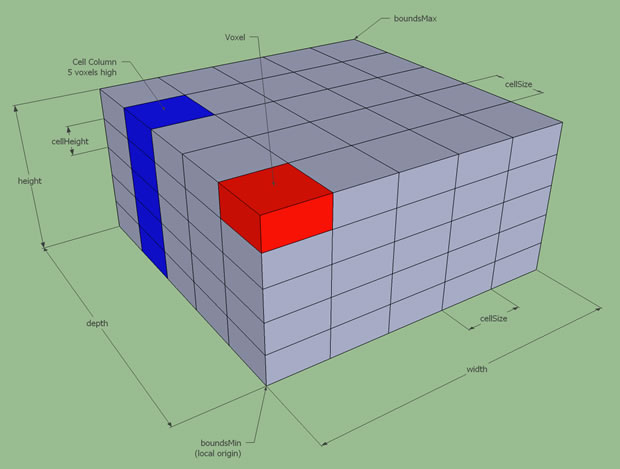
\includegraphics[width=1\textwidth]{hf_03_voxelgrid.png}
	\caption{A voxel grid}
\end{figure}
  
  \item\textbf{Region Generation}: Detect the top surface area of the solid height-field and divide it up into regions of contiguous spans;

  
  
  \begin{figure}[H]
        \centering
        \begin{subfigure}[b]{0.48\textwidth}
                \centering
                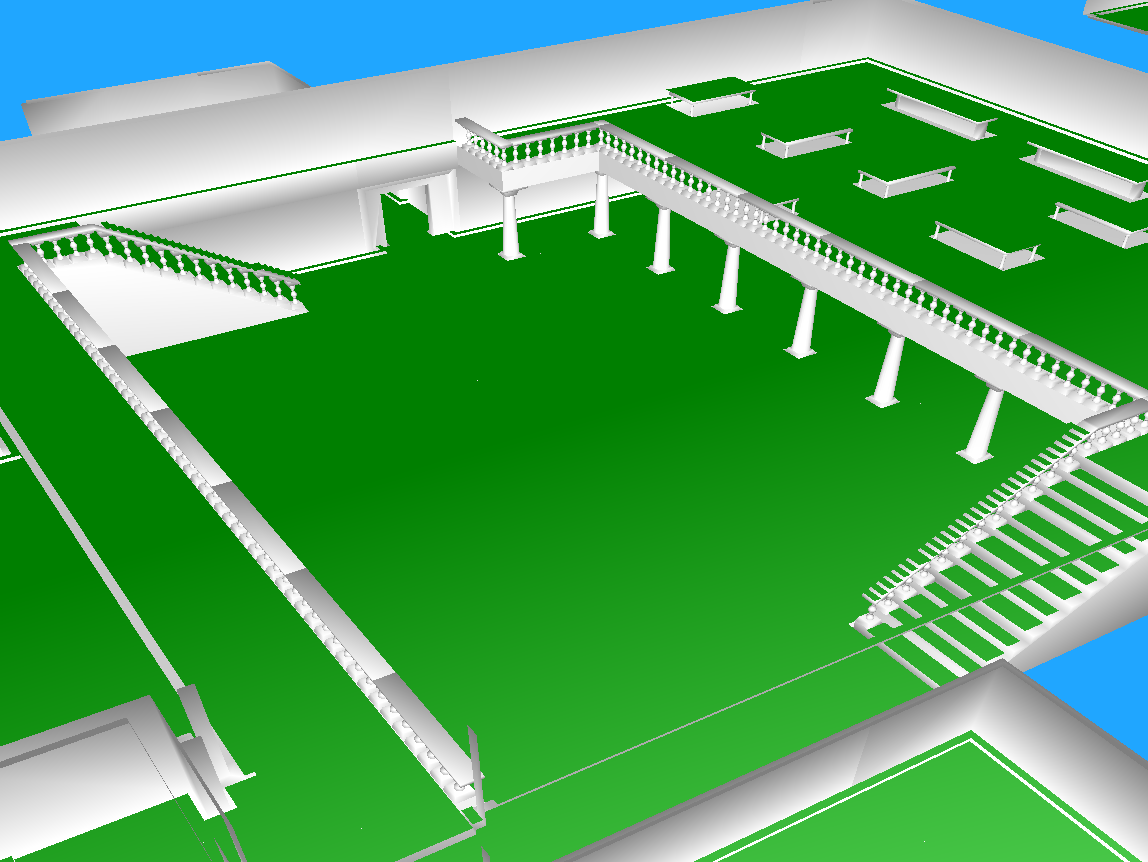
\includegraphics[width=\textwidth]{region_generation.png}
                \caption{Overview of the model}
        \end{subfigure}
        \begin{subfigure}[b]{0.48\textwidth}
                \centering
                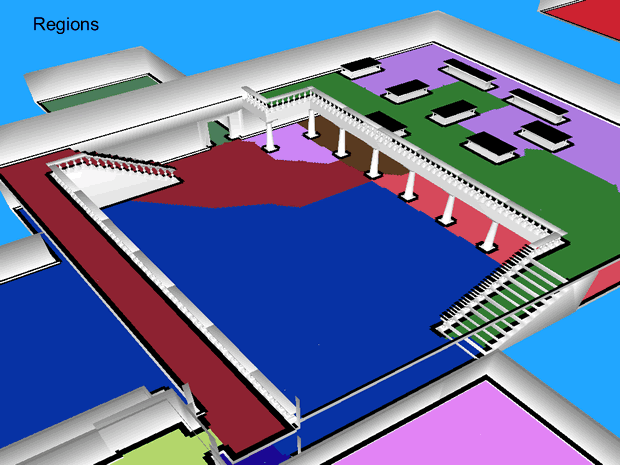
\includegraphics[width=\textwidth]{stage_regions.png}
                \caption{Model split into regions}
        \end{subfigure}
        \caption{Region generation}
	\end{figure}        

  \item\textbf{Contour Generation}: Detect the contours of the regions and form them into simple polygons;

  
  \item\textbf{Convex Polygon Generation}:  Sub-divide the contours into convex polygons;
  
  \begin{figure}[H]
        \centering
        \begin{subfigure}[b]{0.48\textwidth}
                \centering
                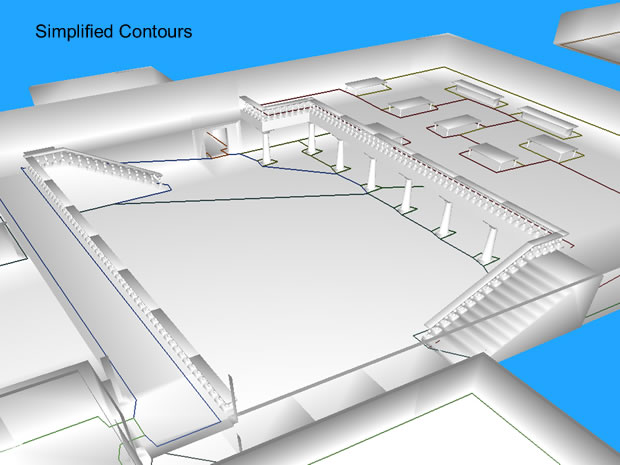
\includegraphics[width=\textwidth]{cont_11_simplified_full.png}
                \caption{Contour generation}
        \end{subfigure}
        \begin{subfigure}[b]{0.48\textwidth}
                \centering
                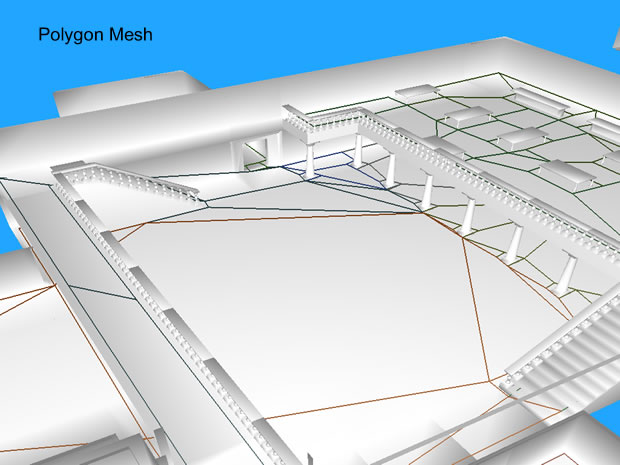
\includegraphics[width=\textwidth]{stage_polygon_mesh.png}
                \caption{Convex polygon division}
        \end{subfigure}
        \caption{Region generation}
	\end{figure}   
  
  
  
  
  
  \item\textbf{Detailed Mesh Generation}: Triangulate the polygon mesh and add height detail.
  
  \begin{figure}[H]
	\centering
	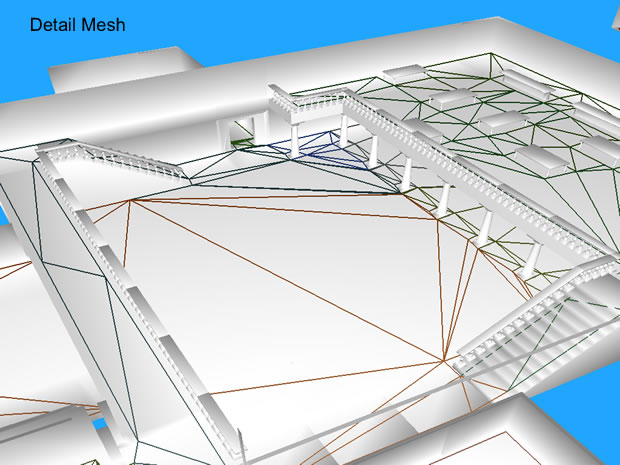
\includegraphics[width=1\textwidth]{stage_detail_mesh.png}
	\caption{Detailed mesh}
\end{figure}  
  
\end{enumerate}


In order to obtain a well-formed mesh, several parameters are required to be passed to the generator (note: where parameters are dependent on variables like agent surface area or agent height, the corresponding values should be calculated in relation to the scale of the imported model):
\begin{itemize}
  \item\textbf{Cell size}: Represents the width and depth of the voxel units which will fill the source geometry. This parameter will influence the accuracy of the generated navigation mesh in relation to the supplied geometry mesh. Lower values closely make the result closely match the source geometry but with a proportional increase in computation time and space costs. In order for the navmesh to be well-formed, this parameter needs to be at least several times smaller than the size of an agent's surface area.
  
  \item\textbf{Cell height}: Represents the height of the voxels used to create the solid height-field. Like the width and depth, the height of the voxel influences the level of accuracy of the navmesh. A well-formed navmesh requires this parameter to be at least several times smaller than the height of an agent's maximum step (step-height).
  
\begin{figure}[H]
	\centering
	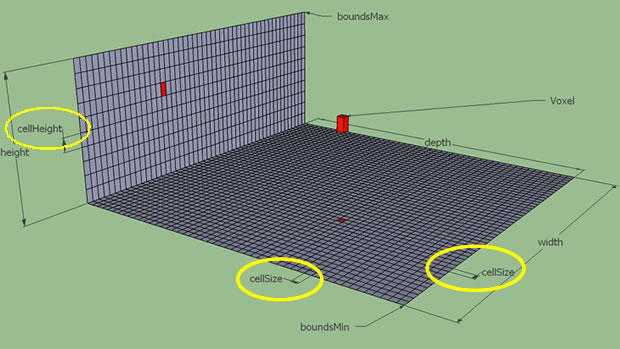
\includegraphics[width=1\textwidth]{cell_size_height.png}
	\caption{Cell size and height}
\end{figure}   

  
  \item\textbf{Minimum traversable height}: Represents the minimum distance from the floor to the ceiling that will still allow an agent to pass through. Should be at least the size of maximum agent height. Should also be at least two times the height of a voxel (cell height).
  
  \begin{figure}[H]
	\centering
	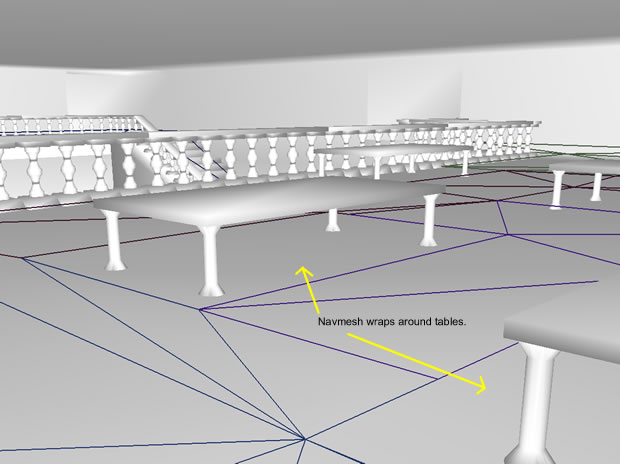
\includegraphics[width=1\textwidth]{main_walkheight_norm.png}
	\caption{When minimum traversable height set correctly, the mesh does not flow under the tables}
\end{figure}   
  
  \item\textbf{Maximum traversable step}:  Represents the maximum height of a ledge that can be climbed by an agent. Should be at least twice the height of a voxel.
  
\begin{figure}[H]
	\centering
	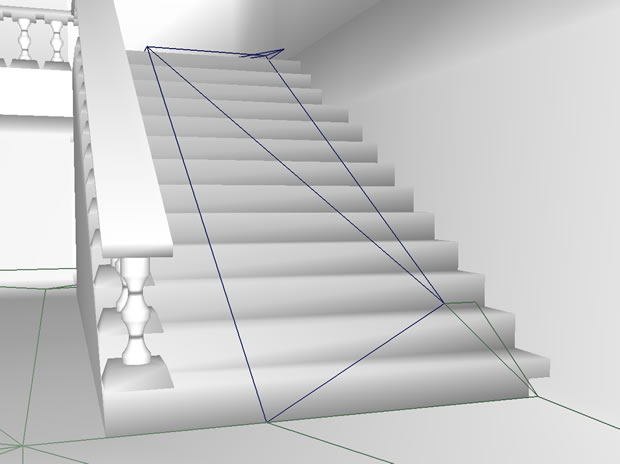
\includegraphics[width=1\textwidth]{max_trav_step.png}
	\caption{Setting a correct value for the maximum traversable step, elements such as stairs can be detected and made walkable}
\end{figure} 
  
  \item\textbf{Maximum traversable slope}: Represents the maximum slope of a ramp that is still considered traversable. Any ramps with a higher slope will be considered unwalkable and will be considered an obstacle by the navmesh.
  
  \item\textbf{Border size of traversable area}: Represents the distance from the walls to the actual walkable area. For a well-formed navmesh, this should be at least the same size as an agent's surface area.
  
	\begin{figure}[H]
	\centering
	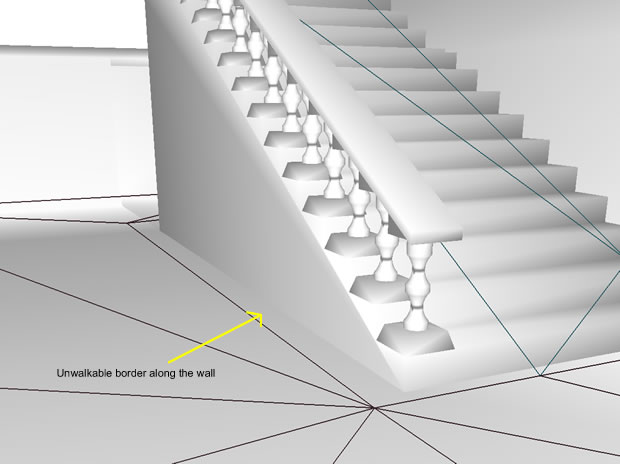
\includegraphics[width=1\textwidth]{border_trav_size.png}
	\caption{The walkable surface will be limited to at least the size of the border. Setting the border size to at least the size of an agent's surface area enables the agent to be positioned on any point of the mesh, without worrying of contact with the walls}
\end{figure} 

  
  \item\textbf{Smoothing threshold}: The amount of smoothing (larger region size, fewer thin triangles) to be performed when generating the distance field
  
%  	\begin{figure}[H]
%	\centering
%	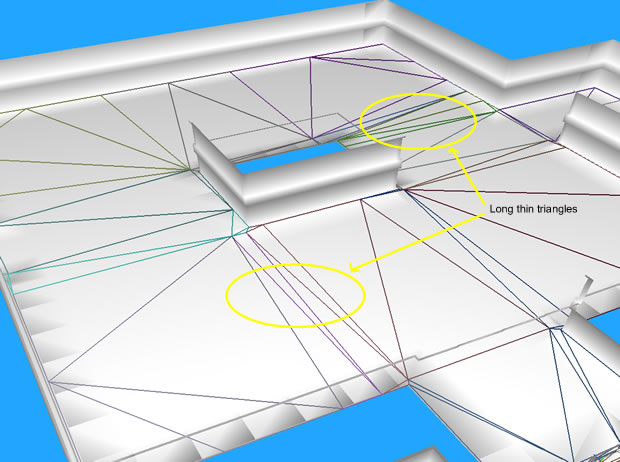
\includegraphics[width=1\textwidth]{smoothing_0.png}
%	\caption{Smoothing disabled}
%\end{figure}
%
% 	\begin{figure}[H]
%	\centering
%	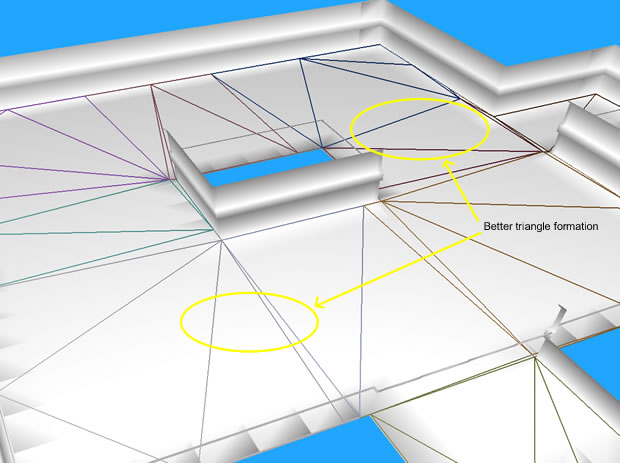
\includegraphics[width=1\textwidth]{smoothing_1.png}
%	\caption{Smoothing enabled}
%\end{figure}  


\begin{figure}[H]
        \centering
        \begin{subfigure}[b]{0.48\textwidth}
                \centering
                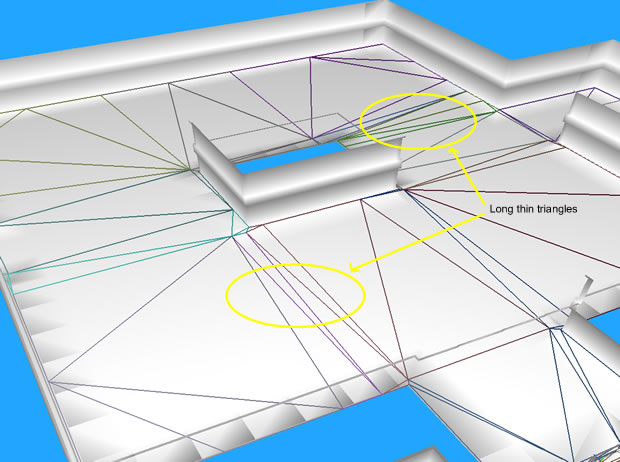
\includegraphics[width=\textwidth]{smoothing_0.png}
                \caption{Smoothing disabled}
        \end{subfigure}
        \begin{subfigure}[b]{0.48\textwidth}
                \centering
                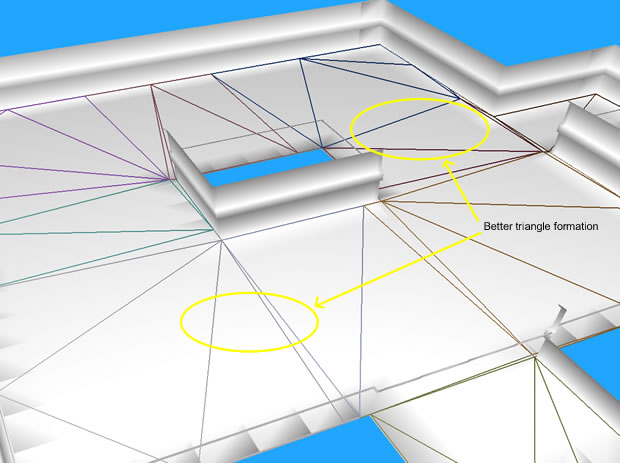
\includegraphics[width=\textwidth]{smoothing_1.png}
                \caption{Smoothing enabled}
        \end{subfigure}
        \caption{Smoothing threshold}
	\end{figure}        

  
  \item\textbf{Minimum size of unconnected region}: Represents the surface, in voxels, of regions that should not be added to the navmesh if they are unconnected to other regions (i.e. islands).
  
  

\begin{figure}[H]
        \centering
        \begin{subfigure}[b]{0.49\textwidth}
                \centering
                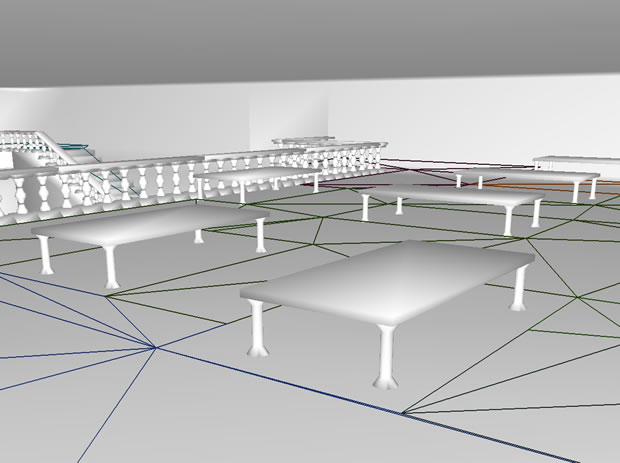
\includegraphics[width=\textwidth]{min_unconn_region_0.png}
                \caption{A correct value for the minimum unconnected region size does not create a mesh surface for the table tops}
        \end{subfigure}
        \begin{subfigure}[b]{0.49\textwidth}
                \centering
                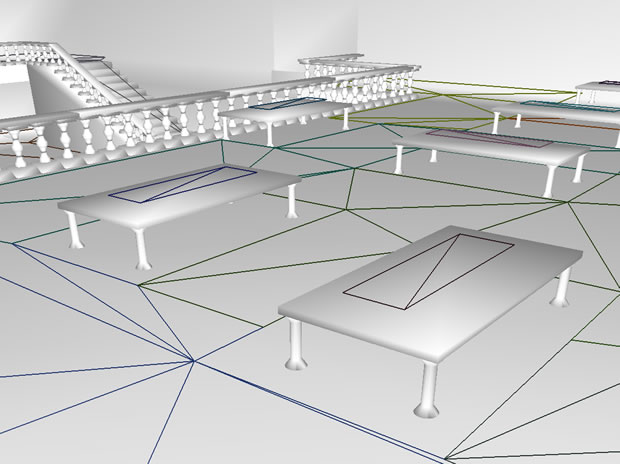
\includegraphics[width=\textwidth]{min_unconn_region_1.png}
                \caption{Setting the value of the minimum unconnected region size too low, the table tops are interpreted as walkable surfaces}
        \end{subfigure}
        \caption{Minimum unconnected region size}
	\end{figure}        


  
%  \begin{figure}[H]
%	\centering
%	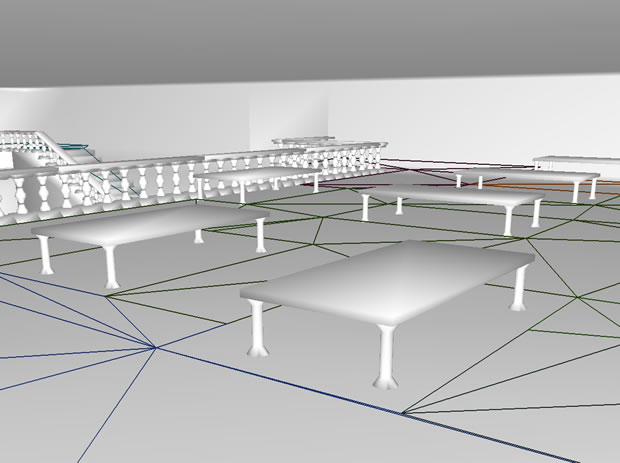
\includegraphics[width=1\textwidth]{min_unconn_region_0.png}
%	\caption{A correct value for the minimum unconnected region size does not create a mesh surface for the table tops}
%\end{figure}
%  
%  \begin{figure}[H]
%	\centering
%	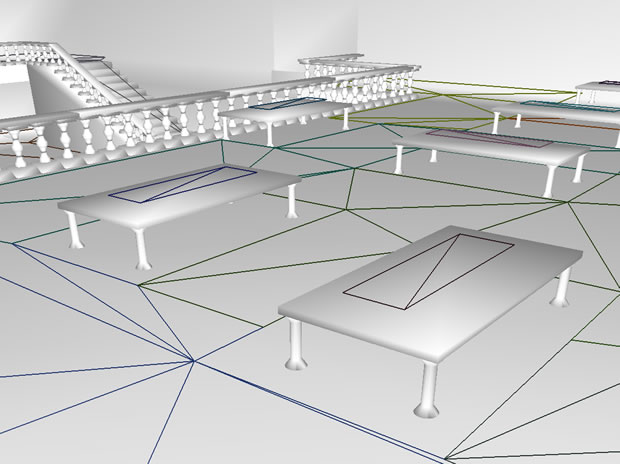
\includegraphics[width=1\textwidth]{min_unconn_region_1.png}
%	\caption{Setting the value of the minimum unconnected region size too low, the table tops are interpreted as walkable surfaces}
%\end{figure}
  
  \item\textbf{Merge region size}: Represents the minimum number of voxels a region should have in order to not try and merge it with other adjacent regions. This influences the number of long thin regions.
  
  \begin{figure}[H]
	\centering
	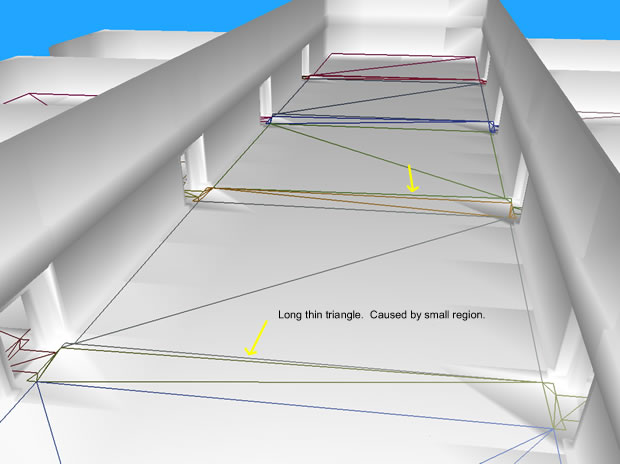
\includegraphics[width=1\textwidth]{merge_region_0.png}
	\caption{With merge region size set too low, the surfaces can be covered by a large number of long thin triangles}
\end{figure}
  
  \begin{figure}[H]
	\centering
	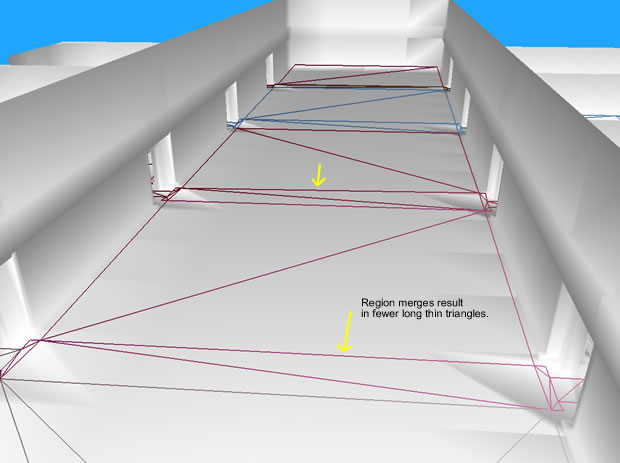
\includegraphics[width=1\textwidth]{merge_region_1.png}
	\caption{Setting the merge region size to a large enough value, some of the thin triangles are merged together with adjacent triangles (where possible)}
\end{figure}
  
  \item\textbf{Maximum edge length}: Represents the maximum length of a triangle's edge. If a triangle has a greater length, it will be split into several legal triangles, by adding more vertices on the border edges.
  
  \begin{figure}[H]
	\centering
	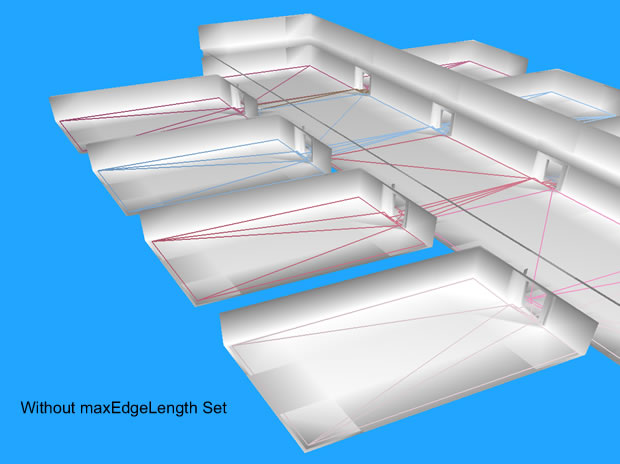
\includegraphics[width=1\textwidth]{max_edge_0.png}
	\caption{With the maximum edge length setting disabled, very long triangles can be generated}
\end{figure}

  \begin{figure}[H]
	\centering
	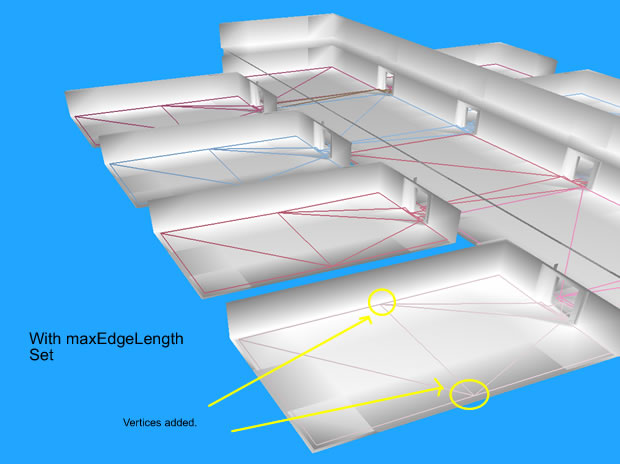
\includegraphics[width=1\textwidth]{max_edge_1.png}
	\caption{With the maximum edge length setting enabled, more vertices are added along the edge of the initial long triangles}
\end{figure}
  
  \item\textbf{Edge maximum deviation}: Influences the accuracy of the edges following the source geometry. The lower the value, the higher the accuracy, but at increased triangle count and processing cost.
  
  \begin{figure}[H]
	\centering
	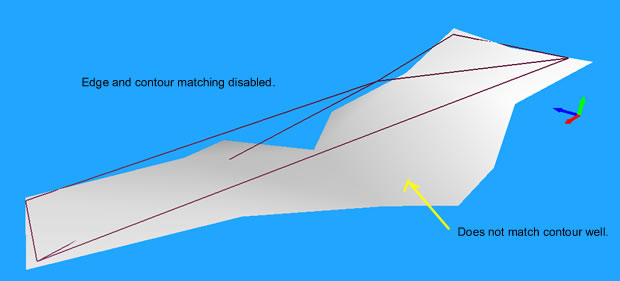
\includegraphics[width=1\textwidth]{edge_dev_0.png}
	\caption{Edge maximum deviation disabled}
\end{figure}
\begin{figure}[H]
	\centering
	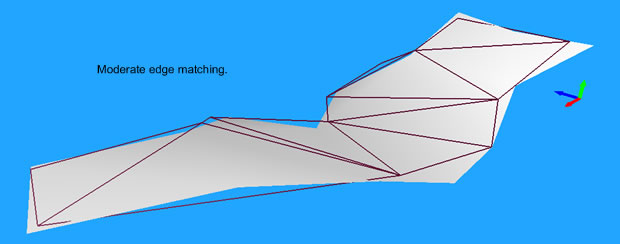
\includegraphics[width=1\textwidth]{edge_dev_1.png}
	\caption{Moderate edge matching}
\end{figure}
\begin{figure}[H]
	\centering
	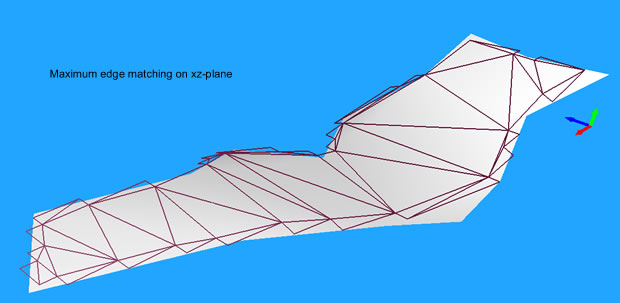
\includegraphics[width=1\textwidth]{edge_dev_2.png}
	\caption{Higher fidelity edge matching}
\end{figure}
  
  
  \item\textbf{Max vertex per polygon}: If set to higher than 3, increases the cost of the computation but can result in better formed regions. However, for the current project, a value of 3 should be used, since the algorithms designed for path-finding only support 3-sided cells.
\end{itemize}
	

The problem that arises with such a high number of variables is the fact that end-users will not be able to import new models from different evacuation environments without a significant overhead. If wrong parameters are used for the mesh generation, the set of algorithms used might generate badly formed meshes, which do not map the source environment closely enough or even fail all-together.
Still, with proper scaling of the model, either in blender stage or after importing the geometrical mesh, importing models of different magnitudes can be achieved.
Since the space available for this report is limited, navigation mesh generation was presented only succinctly. For more in-depth information about each of the steps taken and how the previously discussed parameters influence the resulted mesh, the reader can refer to the NMGen Project documentation. {reference}
\section{Navigation}

\subsection{Logical structure}

\begin{figure}[H]
	\centering
	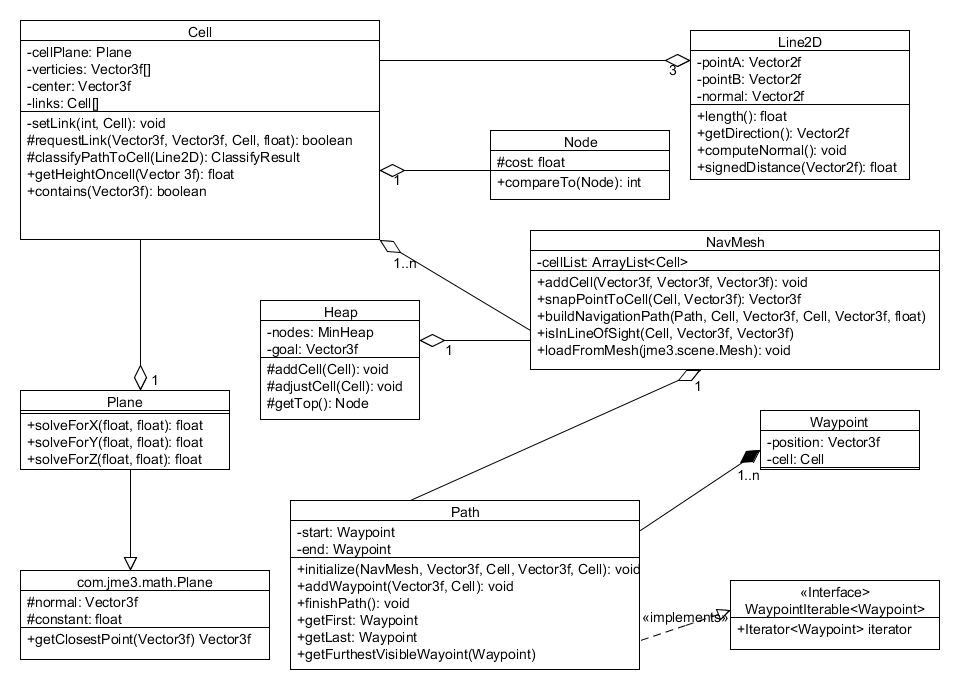
\includegraphics[width=1\textwidth]{navmesh.png}
	\caption{Navmesh Package}
\end{figure}

some text

\subsection{Pathfinding}
  
lala 2

\end{document}
